\documentclass[../main.tex]{subfiles}

\begin{document}

\section{Fysica voorbij het Standaard Model}%
\label{sec:fysica_voorbij_het_standaard_model}

\subsection{Het standaard Model: wat zit daar nu allemaal in?}%
\label{sub:het_standaard_model_wat_zit_daar_nu_allemaal_in_}

\begin{equation}
    \begin{aligned}
        \label{eq:standaard_model}
            \begin{array}{ccc}
                \left(\begin{array}{c}
                        \nu_{e} \\
                        e
                        \end{array}\right) & \left(\begin{array}{c}
                        \nu_{\mu} \\
                        \mu
                        \end{array}\right) & \left(\begin{array}{c}
                        \nu_{\tau} \\
                        \tau
                \end{array}\right) \\
                \left(\begin{array}{l}
                        u \\
                        d
                        \end{array}\right) & \left(\begin{array}{l}
                        c \\
                        s
                        \end{array}\right) & \left(\begin{array}{l}
                        t \\
                        b
                \end{array}\right)
            \end{array}\\
            \gamma, W^{+}, W^{-}, Z, g, H
    \end{aligned}
\end{equation}
Dit zijn alle deeltjes die nodig hebben om het Standaard Model te laten werken. Deze zijn ook allemaal gevonden.\\
Waarom beperken we ons hier tot 4 generaties (Dit moet omdat de $CP$ schending niet meer zou kloppen), zijn er nog andere uitwisselingdeeltjes, zijn er nog andere interacties, zijn er parameters die we nog niet kennen?

\subsection{4de generatie fermionen}%
\label{sub:4de_generatie_fermionen}

\subsubsection{Leptonen}%
\label{ssub:leptonen}

Indien we een vierde generatie leptonen zouden hebben zou de massa van de 4de generatie groter moeten zijn dan $45$GeV. Voor de geladen leptonen weten we dat $m_l > 101$GeV omdat we nog geen resonantie zijn tegen gekomen in $e^{+} e^{-} \rightarrow l^{+} l^{-}$ tot $\sqrt{s}=209 \mathrm{GeV}$.

\subsubsection{Quarks}%
\label{ssub:quarks}

Uit de unitariteit van de CKM-matrix is het duidelijk dat daar niet veel zal zitten. We doen hier ook direct onderzoek naar op het LHC maar er is nog niets gevonden.

\begin{figure}[h]
    \centering
    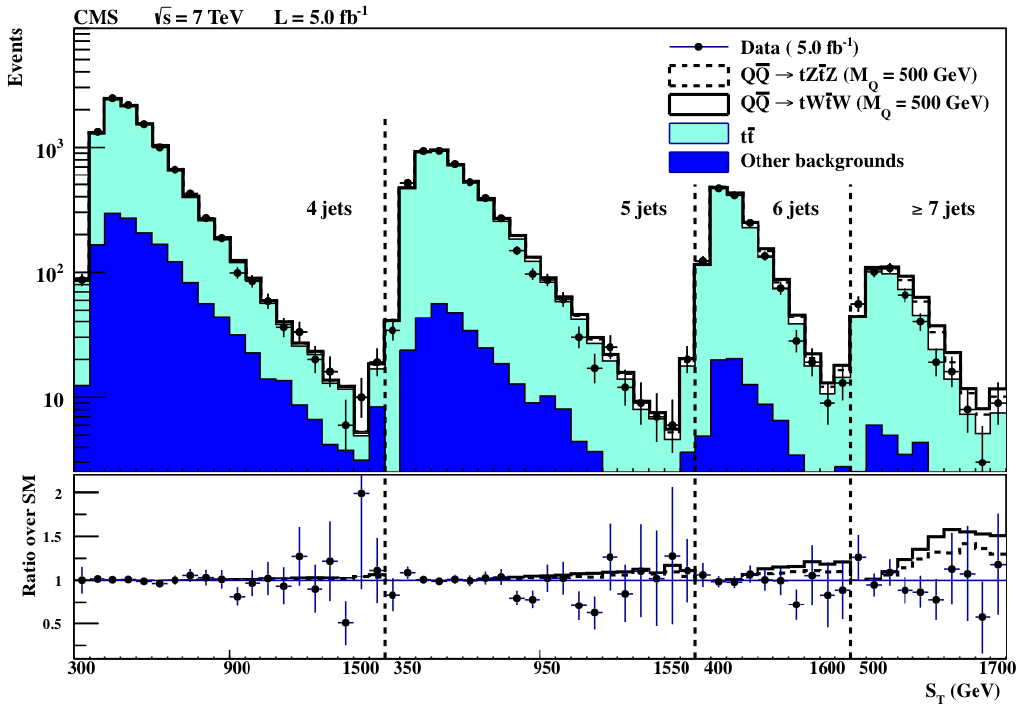
\includegraphics[width=0.6\linewidth]{physics_beyond_the_standard_model/lhc_4_gen_zoektocht.png}
    \caption{Zoektocht naar 4de generatie quarks in LHC}%
    \label{fig:physics_beyond_the_standard_model/lhc_4_gen_zoektocht}
\end{figure}

Uit de proton proton botsingen kunnen zowel 4, 5, 6 of 7 jets komen. Berekenen we alle mogelijke productie kanalen van deze jets zien we dat we bij de metingen niet echt afwijken van de voorspellingen. Er zit daar dus niet echt een 4de generatie aan quarks.

\subsection{Nieuwe uitwisseling bosonen}%
\label{sub:nieuwe_uitwisselings_bosonen}

Waarom zouden er geen extra $W'$ en $Z'$ bosonen bestaan. Misschien koppelen deze aan rechtshandige fermionen. Wie weet is $Z$ een samengestelde toestand en is daar een aangeslagen toestand van.

\begin{figure}[h]
    \centering
    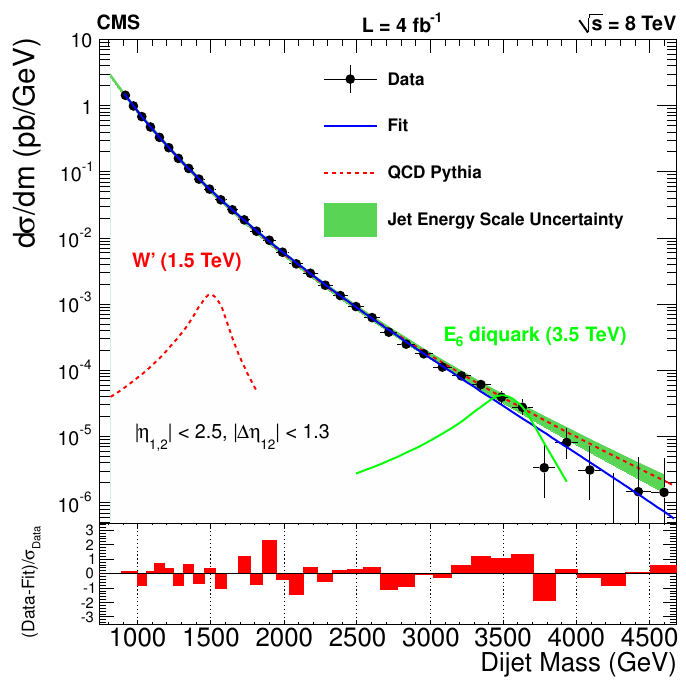
\includegraphics[width=0.4\linewidth]{physics_beyond_the_standard_model/cms_w'_z'_zoektocht.png}
    \caption{Zoektocht naar $W'$ en $Z'$ in LHC}%
    \label{fig:physics_beyond_the_standard_model/cms_w'_z'_zoektocht}
\end{figure}

We gaan kijken hier naar 2 jet fenomenen waar we hun gecombineerde massa uitzetten in vergelijking tot de werkzame doorsnede. De groene lijn is wat we verwachten en de blauwe lijn is wat we meten. We zien hier niet de spectra indien een $W'$ of diquark zou bestaan. Er is dus geen ruimte om af te wijken van het standaard model hier. Hetzelfde kunnen we vinden als we kijken naar de elektron positron vervallen. Er is hier ook geen plaats om de nieuwe intermediaire deeltjes toe te voegen aan het model.

\begin{figure}[h]
    \centering
    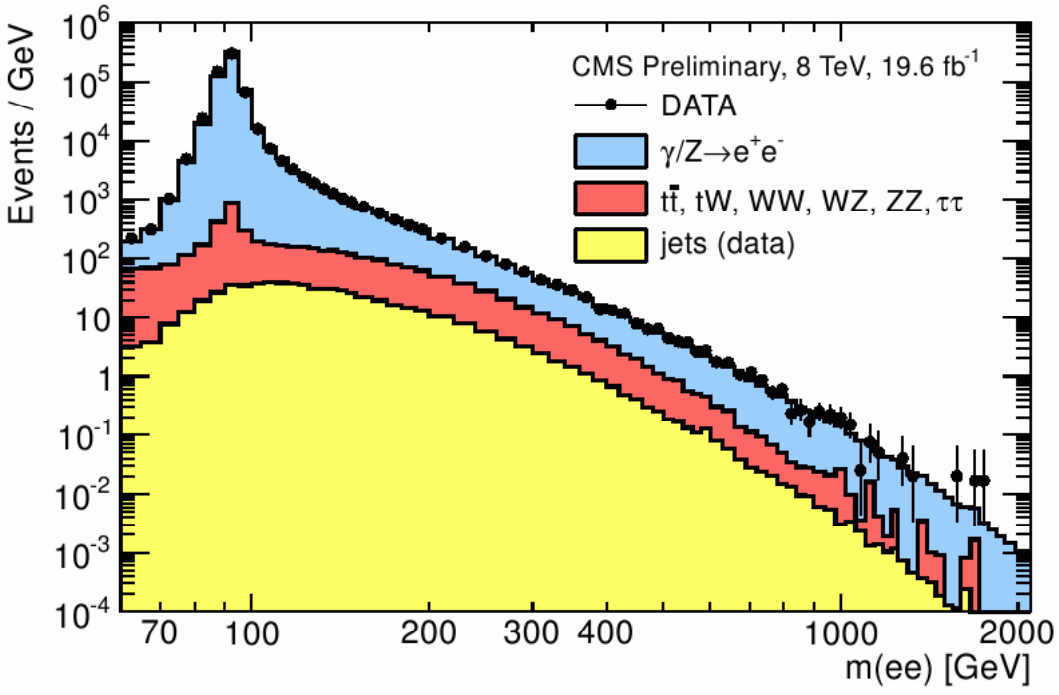
\includegraphics[width=0.6\linewidth]{physics_beyond_the_standard_model/ee_w'_z'_zoektocht.png}
    \caption{Zoektocht naar $W'$ en $Z'$ in LHC aan de hand van elektronen en positronen}%
    \label{fig:physics_beyond_the_standard_model/ee_w'_z'_zoektocht}
\end{figure}

\subsection{Zwarte gaten}%
\label{sub:zwarte_gaten}

Het is nu ook mogelijk om te zoeken naar zwarte gaten. Deze worden voorspelt door string theory. Deze voorspelt dat er nog veel meer dimensies zijn. In de opgerolde dimensies zou de zwaartekracht veel groter moeten zijn. Indien we deze dimensies zouden beginnen raken als we onze deeltjes maar dicht genoeg tot elkaar brengen zou het mogelijk moeten zijn om mini zwarte gaten te kunnen maken.
\begin{equation}
    \begin{aligned}
        \label{eq:zwarte_gaten}
        p p \rightarrow B H+X
    \end{aligned}
\end{equation}
Deze zijn heel klein en zouden zo goed als instant vervallen (verdampen) aan de hand van Hawking radiatie. Bij het maken van deze zwarte gaten zou een hoge multipliciteit aan finale toestanden moeten zijn van veel jets en leptonen. Om dit te onderzoeken kijken we of we zo evenementen kunnen vinden met grote jet aantallen.
\begin{figure}[h]
    \centering
    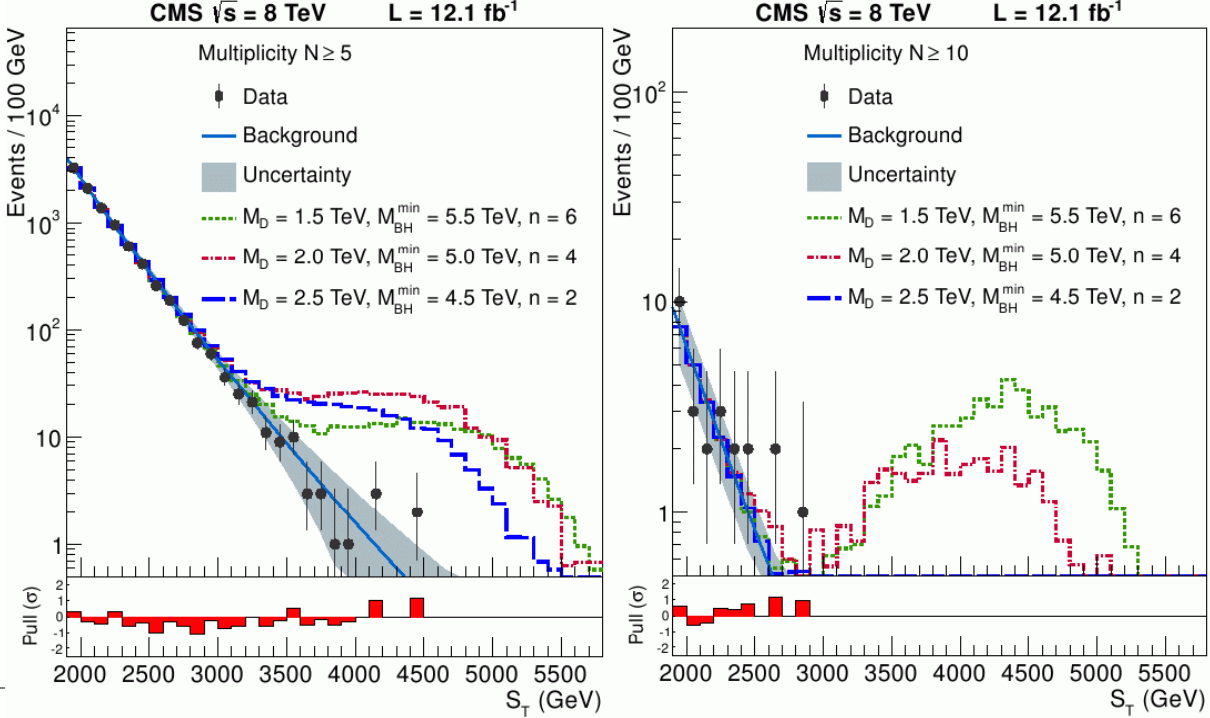
\includegraphics[width=0.6\linewidth]{physics_beyond_the_standard_model/zwarte_gaten.png}
    \caption{Zoektocht naar zwarte gaten}%
    \label{fig:physics_}
\end{figure}

In het blauw kan je de verwachtingen zien wat perfect zal kloppen met wat we zien. Indien we zwarte gaten zouden hebben met de massa's gegeven in de grafieken zouden we een grotere hoeveelheid aan evenementen verwachten bij grote $S_T$.

\subsection{Huidige toestand van direct onderzoek}%
\label{sub:huidige_toestand_van_direct_onderzoek}

Op dit moment hebben we nog niets gevonden maar kunnen mogelijke uitbreidingen van het standaard model uitsluiten tot op bepaalde hoeveelheden energie kunnen uitsluiten.

\begin{figure}[h]
    \centering
    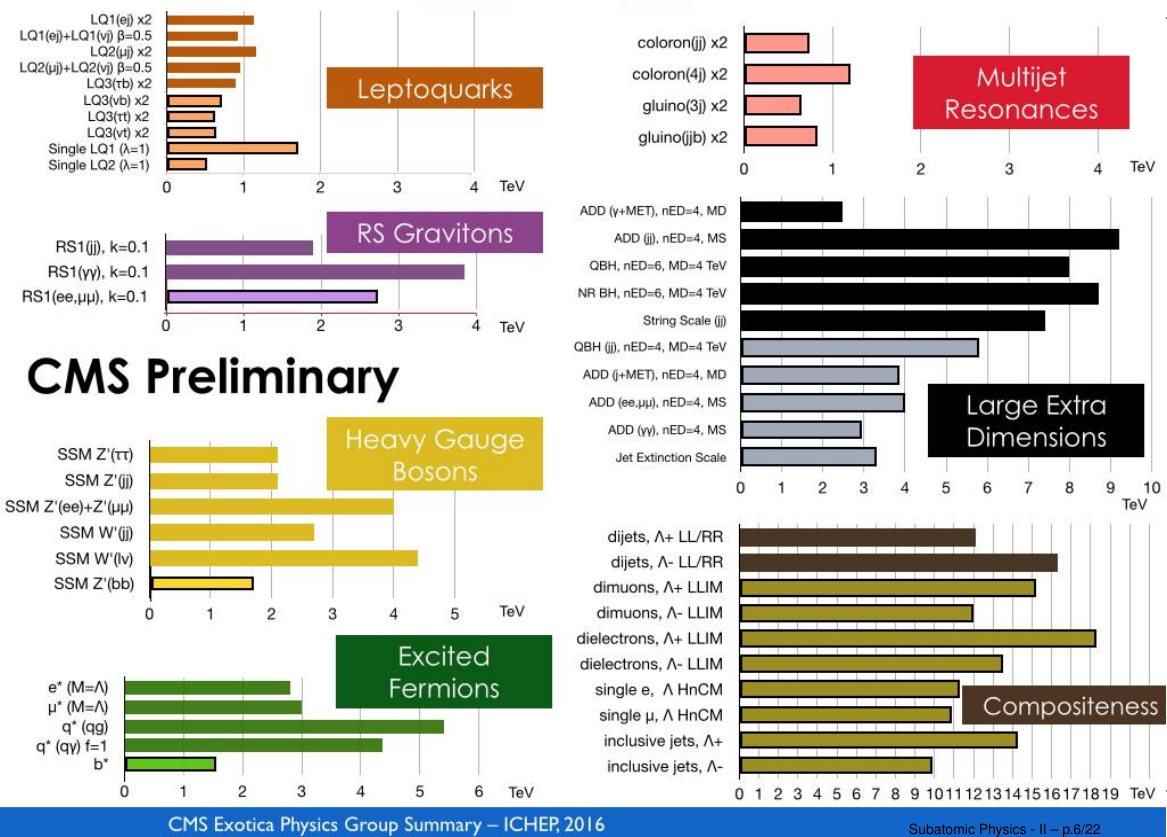
\includegraphics[width=0.6\linewidth]{physics_beyond_the_standard_model/current_state.png}
    \caption{Huidige toestand op deeltjes voorbij het Standaard Model}%
    \label{fig:physics_beyond_the_standard_model/current_state}
\end{figure}

Uiteindelijk is het een zoektocht naar hints die ons verder kunnen helpen in de zoektocht naar een meer complete theorie.

\subsection{Standaard Model}%
\label{sub:standaard_model}

Is het standaard model nu het ultieme model voor de wereld? Dat zou mogelijk kunnen zijn. Hierbij beschrijft de Dirac vergelijking de fermionen, QFT de interacties tussen de deeltjes. De interacties worden afgeleid uit een lokaal ijk principe. Het Higgs mechanisme om elektrozwakke symmetrie te breken en op die manier massa te creëren. Het ongemakkelijke in dit model is dat we al die parameters experimenteel moeten bepalen. Dit beschrijft alles wat we waarnemen, op enkele plaatsen zit daar spanning op maar hebben nog nooit een duidelijke afwijking gezien van het standaard model.\\
Al deze eigenschappen zijn er in gestoken. We weten hoe de Lagrangiaan er uit ziet maar niet waarom deze zo is. Wat we nu aan het onderzoeken zijn is waarom het Standaard model er zo uit ziet.\\
Wat zijn al deze vrije parameters nu in dit Standaard Model.
\begin{table}[h]
    \begin{minipage}[c]{0.48\textwidth}
        \centering
        \caption{Fermion sector}
        \label{tab:fermion_sector_parameters}
        \begin{tabular}{ccc}
            $m_{\nu_{1}}$   & $m_{\nu_{2}}$ & $m_{\nu_{3}}$ \\
            $m_{e}$         & $m_{\mu}$     & $m_{\tau}$ \\
            $m_{d}$         & $m_{s}$       & $m_{b}$ \\
            $m_{u}$         & $m_{c}$       & $m_{t}$
        \end{tabular}
        
        \caption{Ijk sector}
        \label{tab:ijk_sector}
        \begin{tabular}{ccc}
            $\alpha$ & $G_F$ & $\alpha_S$
        \end{tabular}
    \end{minipage}
    \begin{minipage}[c]{0.48\textwidth}
        \centering
        \caption{CKM, PMNS sector}
        \label{tab:ckm_pmns_sector}
        \begin{tabular}{cccc}
            $\lambda$       & $A$           & $\rho$        & $\eta$ \\
            $\theta_{12}$   & $\theta_{13}$ & $\theta_{23}$ & $\delta$
        \end{tabular}
        
        \caption{Higgs sector}
        \label{tab:higgs_sector}
        \begin{tabular}{cc}
            $v$ & $m_H$
        \end{tabular}

        \caption{QCD CP schending}
        \label{tab:qcd_cp_schending}
        \begin{tabular}{cc}
            $\theta_{CP}$
        \end{tabular}
    \end{minipage}
\end{table}

Indien er maar 1 van deze parameters er een beetje anders zou uit zien dan zou het heelal er totaal anders uit zien. De 26ste parameter, de $CP$ schending van de sterke wisselwerking is de enige die we nog niet hebben waargenomen.

\subsection{Behouden grootheden}%
\label{sub:behouden_grootheden}

In de ruimte-tijd symmetrieën hebben we het behoud van energie, impuls, draaimoment en pariteit. We zijn vrij zeker dat deze allemaal behouden worden binnen de beperkingen van het heisenberg principe. Het behoud van lading, zwakke lading en kleur zijn telkens overeen komen met een ijkveld, een veld symmetrie. Het Baryon getal $\mathcal{B}$ wordt blijkbaar behouden tot op zekere hoogte. Anders zou het universum vandaag de dag even veel baryonen als antibaryonen hebben. We zien dat het massa en het baryon getal verbonden zijn met elkaar door een massaloos veld dat eruit ziet als zwaartekracht. Er zit een kleine afwijking tussen het baryon getal en het massagetal vanwege de nucleaire binding. Het onderzoek naar dit massaloos veld is gedaan maar daar is niets gevonden. De koppeling van baryonen aan dit veld zou een stuk kleiner moeten zijn dan de koppeling van de zwaartekracht ($K<10^{-9}G$). Het is dus niet duidelijk waarom het baryon en lepton getal behouden worden in het Standaard Model.\\
Vandaag de dag zien we dat het de sterke interactie $CP$ niet zal schenden, $\theta_{C P} \approx 0$. Hier is geen a priori reden voor.Indien we zien dat iets behouden wordt, zijn we geneigd om daar een nieuw ijkveld aan te hangen, in dit geval een pseudoscalair veld. Indien er een nieuw ijkveld is, wordt er automatisch een nieuw ijkboson toegevoegd. In dit geval is de voorgestelde naam een axion wat een licht ($\sim 1\mu$eV-eV) neutraal pseudoscalair deeltje is. De eigenschappen van dit deeltje zijn slecht bepaald wat niet van belang is. Het moet er gewoon zijn en op een of andere manier koppelt aan de bestaande deeltjes. Dit geeft een lading en zou het $CP$ behoud verklaren. Dit zou dus opmengen met andere pseudoscalaire deeltjes zoals $\pi^0$ en $\eta$ die dan vervallen in 2 fotonen. Dit geeft een koppeling van axionen naar 2 fotonen. Het fuseren van 2 fotonen in een axion kan gebruikt worden om daar onderzoek naar te doen.

\begin{figure}[h]
    \centering
    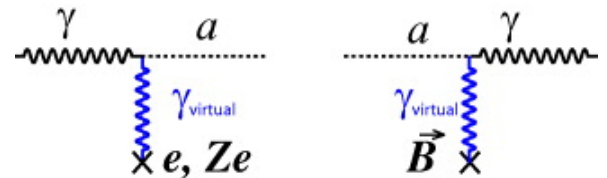
\includegraphics[width=0.4\linewidth]{physics_beyond_the_standard_model/axion_diagrammen.png}
    \caption{Feynman diagrammen waar we experimenteel naar op zoek zijn om het axion te vinden.}%
    \label{fig:physics_beyond_the_standard_model/axion_diagrammen}
\end{figure}

Hier annihileert een foton met een virtueel foton uit een magneetveld om een axion te maken dat dan terug in een magneetveld kan vervallen naar 2 fotonen. CAST doet dit onderzoek door fotonen in te laten invallen in een magneet van het LHC. Centraal staat een blok lood die de fotonen zal tegen houden maar niet de aangemaakte axionen die zo goed als niet interageren met materie. Deze axionen interageren achter het loodblok terug met het magneetveld en kijken dan of ze enige fotonen kunnen waarnemen.

\begin{figure}[h]
    \centering
    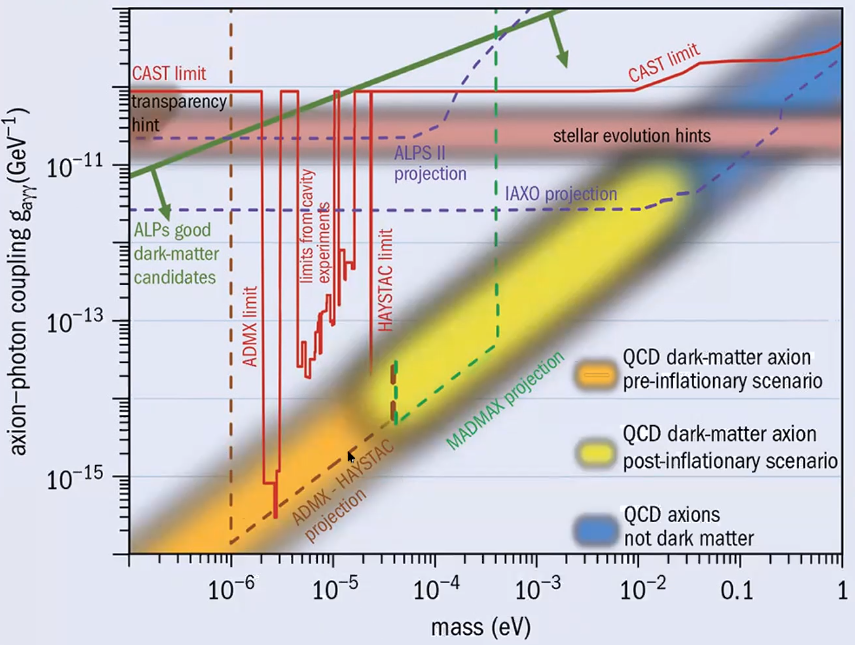
\includegraphics[width=0.6\linewidth]{physics_beyond_the_standard_model/cast_resultaten.png}
    \caption{Resultaten voor het onderzoek naar axionen}%
    \label{fig:physics_beyond_the_standard_model/cast_resultaten}
\end{figure}

Verticaal in de resultaten zichbaar in figuur \ref{fig:physics_beyond_the_standard_model/cast_resultaten} zie je de koppelingsterkte van axionen aan fotonen die niet a priori gegeven is en horizontaal de massa van de axionen. In de blauwe, gele en oranje band geven aan waar het axion zou moeten zitten als de juiste eigenschappen zou moeten hebben om het QCD $CP$ probleem op te lossen. Wat we uit de werking van sterren al kunnen zien is dat de fotonen niet al te sterk mogen koppelen aan de axionen omdat deze anders niet zouden werken zoals ze nu doen. De roze band geeft aan wat mogelijk zal zijn in functie van wat sterren doen. Indien de massa van de axionen iets hoger zou zijn dan is het mogelijk dat deze donkere materie zijn. Eén van de grootste redenen dat we denken dat er nog iets meer is dan het Standaard Model dat we nu kennen is het bestaan van donkere materie. We willen de link kunnen leggen tussen de subatomaire fysica en de astrofysica. Vandaag de dag met het Standaard Model beschrijven we maar 4 a 5\% van de massa van het heelal. Momenteel zijn we nog gelimiteerd in de limieten van onze metingen, we zijn nog niet mogelijk om preciezer te kijken dan de interstellaire limiet. Vandaag zien de uitgesloten gebieden er zo uit:

\begin{figure}[h]
    \centering
    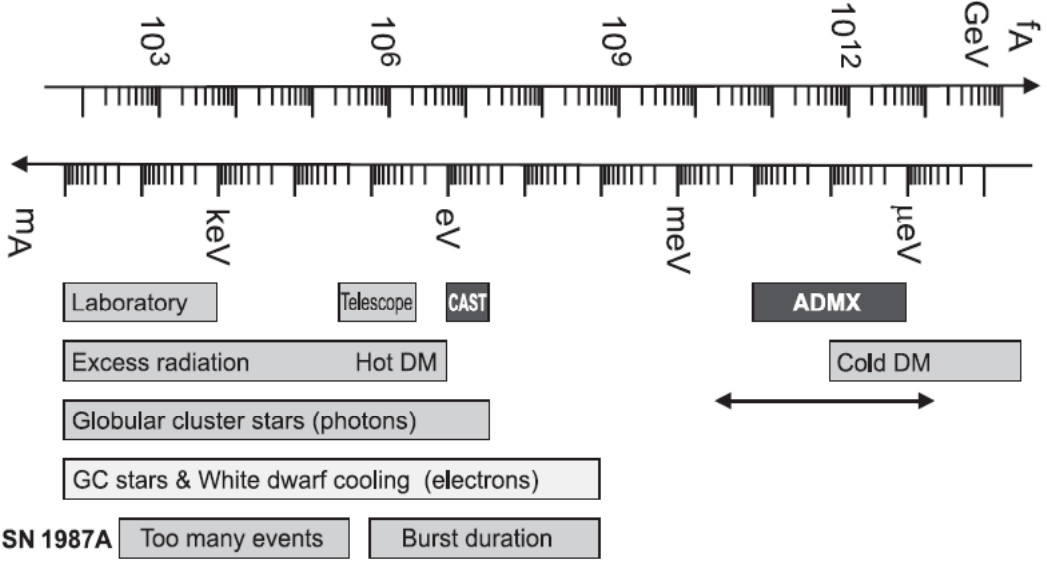
\includegraphics[width=0.6\linewidth]{physics_beyond_the_standard_model/axionen_verboden_gebieden.png}
    \caption{De verboden gebieden van de axionen}%
    \label{fig:physics_beyond_the_standard_model/axionen_verboden_gebieden}
\end{figure}

\subsection{Grand Unified Theories}%
\label{sub:grand_unified_theories}

Voor het uitwisselen van kleine hoeveelheden energie zien we dat de koppelingconstantes van de sterke, zwakke en elektromgnetische wisselwerking grote verschillen tonen. We hebben ook gezien dat dit lopende koppelingconstantes zijn. Voor grotere en grotere hoeveelheden aan energie lijken deze naar elkaar toe te gaan. Extrapoleren we wat we vandaag de dag weten verwachten we bij het uitwisselen van $q=M_{X} \sim 10^{15}$ de krachten even sterk zouden moeten zijn.

\begin{figure}[h]
    \centering
    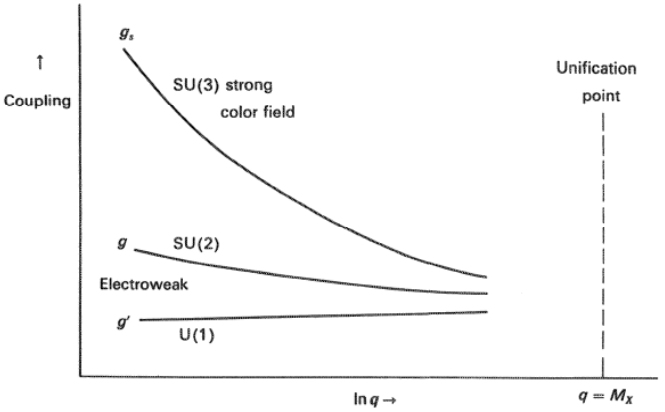
\includegraphics[width=0.5\linewidth]{physics_beyond_the_standard_model/grand_unified_theory.png}
    \caption{Lopende koppelingconstantes in de Grand Unified Theory}%
    \label{fig:physics_beyond_the_standard_model/grand_unified_theory}
\end{figure}

In 1974 waren de eerste ideeën er al om deze krachten te unificeren. Hier zouden ze $SU(1)$, $SU(2)$ en $SU(3)$ samen te brengen tot 1 grotere ijk symmetrie $SU(5)$. Deze $SU(5)$ groep zou zo goed als automatisch uiteen vallen in de 3 groepen die we nu al hebben. Deze theorie zo 24 ijkbosonen bevatten. Deze zijn
\begin{itemize}
    \item 8 gluonen
    \item 3 zwakke bosonen, de $W$ en $Z$ bosonen
    \item het foton
    \item 12 nieuwe ijkbosonen $Y$ en $X$ de leptoquarks
\end{itemize}
Zoals de elektrozwakke symmetrie die wordt gebroken door het Higgs boson zal de Grand Unified Theory symmetrie ook gebroken worden. Deze breuk zou moeten leven bij ongeveer $m_{Y} \sim m_{X} \sim 10^{15}$GeV. Naast de massa van de $Y$ en $X$ bosonen moeten er ook GUT-Higgs bosonen zijn. Uit de theorie zijn de massa van de bosonen gegeven door: $Q_{Y}=-\frac{1}{3}$ en $Q_{X}=-\frac{4}{3}$. Ze hebben naar een lading ook 3 mogelijke kleuren wat in het totaal 12 verschillende mogelijkheden moet geven. Omdat ze een massa hebben zouden deze moeten vervallen in onze deeltjes die we al kennen. Een aantal voorbeelden van zo een vervallen zijn: $X_{1} \rightarrow e^{-} d, \bar{u} \bar{u}$ en $Y_{2} \rightarrow \mu^{-} c, \bar{c} \bar{s}$. De multipletten die we bij deze theorie nu krijgen zijn vrij verschillend, we krijgen hier quintetten en decupletten.
\begin{equation}
    \begin{aligned}
        \label{eq:qut_multipletten}
        \overline{5}&=\left(\begin{array}{c}
                \nu_{e} \\
                e^{-} \\
                \bar{d}_{R} \\
                \bar{d}_{B} \\
                \bar{d}_{G}
        \end{array}\right)_{L H}\\
        10&=\left(\begin{array}{ccccc}
                0 & e^{+} & d_{R} & d_{B} & d_{G} \\
                -e^{+} & 0 & u_{R} & u_{B} & u_{G} \\
                -d_{R} & -u_{R} & 0 & \bar{u}_{G} & \bar{u}_{B} \\
                -d_{B} & -u_{B} & -\bar{u}_{G} & 0 & \bar{u}_{R} \\
                -d_{G} & -u_{G} & -\bar{u}_{B} & -\bar{u}_{R} & 0
        \end{array}\right)_{L H}
    \end{aligned}
\end{equation}
Wat we zien gebeuren is dat de som van de ladingen in de multipletten 0 zal moeten zijn, $\sum_{i} Q_{i}=0$. Dit verklaard waarom we de $-1/3$ en $2/3$ lading hebben voor onze quarks en de gelijkheid $Q(\nu)-Q(e)=Q(u)-Q(d)$.

\end{document}
